\section{Experimental Methodology}
\label{sec:experimentalmethodology}

In this section, we discuss our method for evaluating the performance of the proposed memory systems. We utilize the PARSEC v2.1 benchmark suite with the gem5 simulator to generate memory traces. Next, we run the Ramulator DRAM simulator to to measure the performance of the proposed memory systems. We compare the baseline performance of the Ramulator simulators against a modified version of the Ramulator simulator which implements the proposed memory systems.

\subsection{Memory Trace Generation}

We use the PARSEC benchmark suite to evaluate the performance of the proposed memory systems. The PARSEC benchmark suite was developed for Chip Multiprocessors and is composed of a diverse set of multithreaded applications~\cite{bienia09parsec2}. The benchmarks allow us to observe how the proposed memory systems perform in dense memory access scenarios. A number of input sets are provided alongside the PARSEC benchmarks. To run the PARSEC applications, we use the gem5 simulato~\cite{parsec_2_1_m5}.

The gem5 simulator allows us to select the quantity and attributes of the processors used to generate the memory traces. We used 8 parallel processors for the PARSEC benchmarks we evaluated. The PARSEC applications have a number of regions where the nature of the computation changes. We extract the regions of the trace where the application was performing parallel processing, as it is these regions where there is a high probablity for bank conflicts to occur. 

\Matt{TODO: List the input sets used for each benchmark}

We convert the gem5 memory traces to the Ramulator CPU-trace format. The conversion process is simple as it requires only the reorganization of the memory addresses present in the gem5 memory trace. It is important that we use the Ramulator CPU-trace format and not the DRAM-trace format because the CPU-trace format contains information necessary to simulate the processor subsystem within Ramulator.

\subsection{PARSEC Trace Attributes}

\begin{figure}[htbp]
		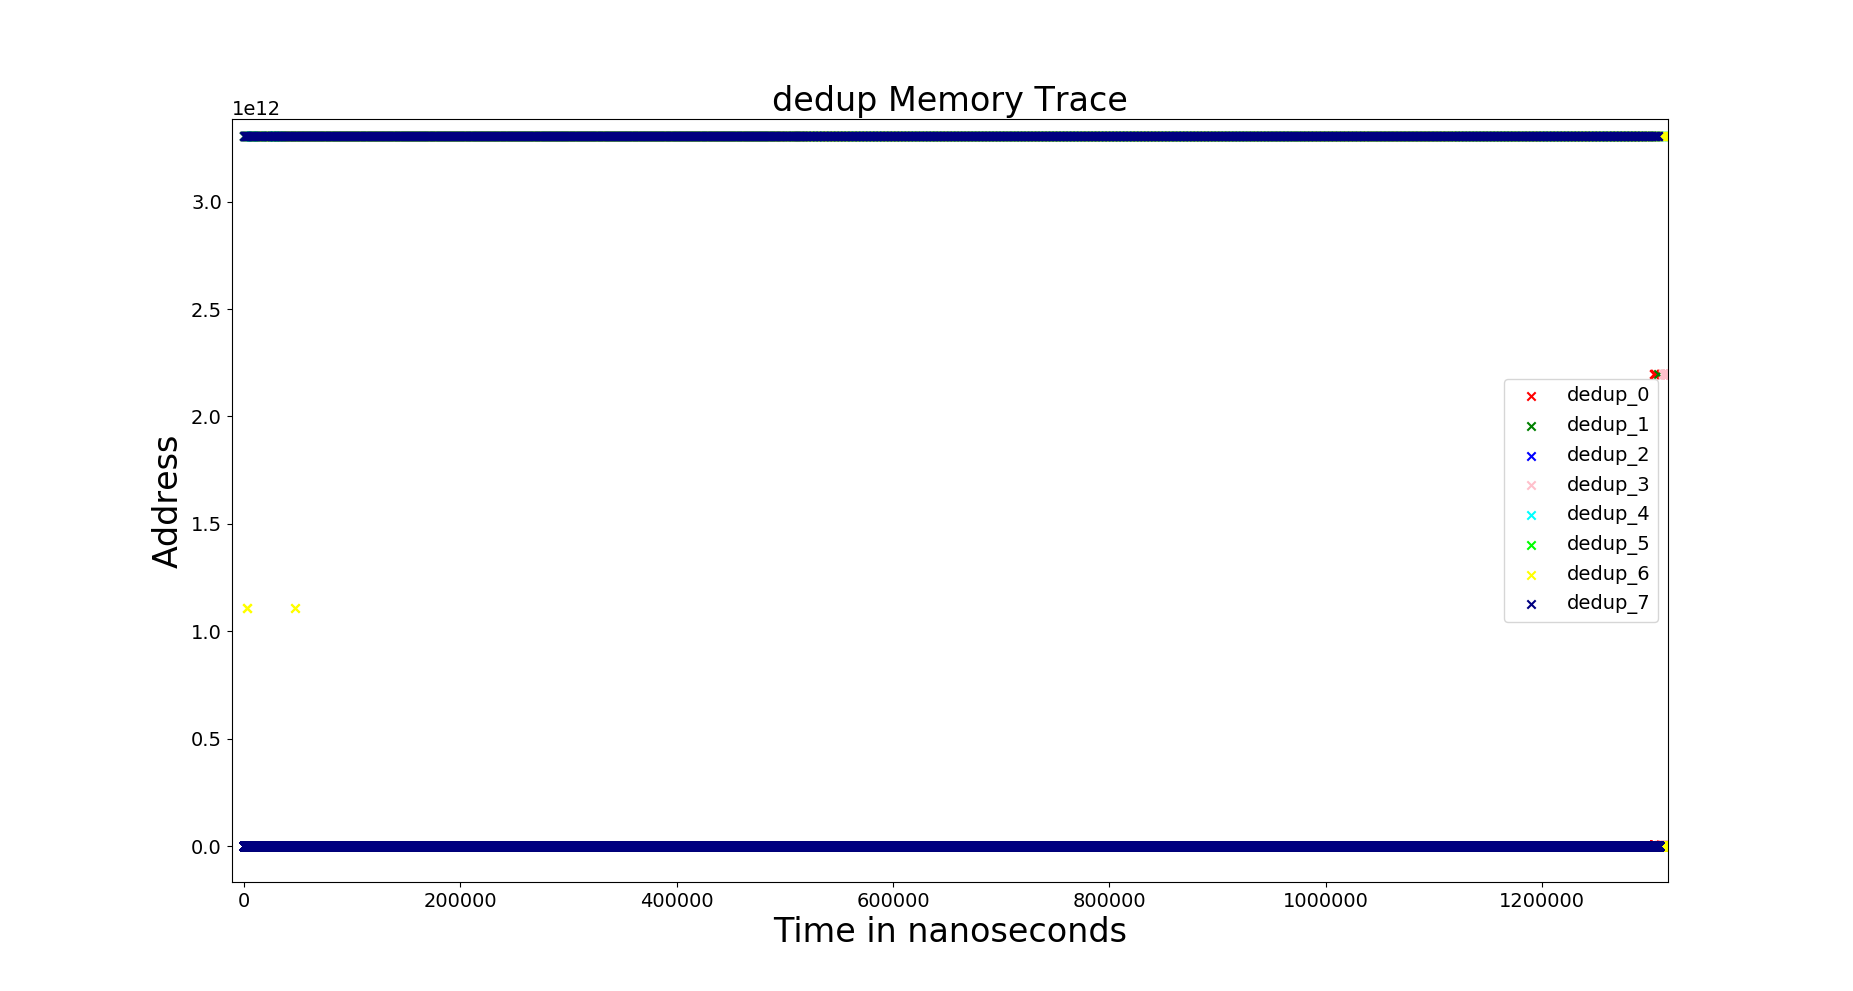
\includegraphics[width=\linewidth]{fig/dedup_whole.png}
		\caption{Memory Access from the Dedup PARSEC benchmark. This trace was generated using 8 cores.}
		\label{fig:dedup_whole}
		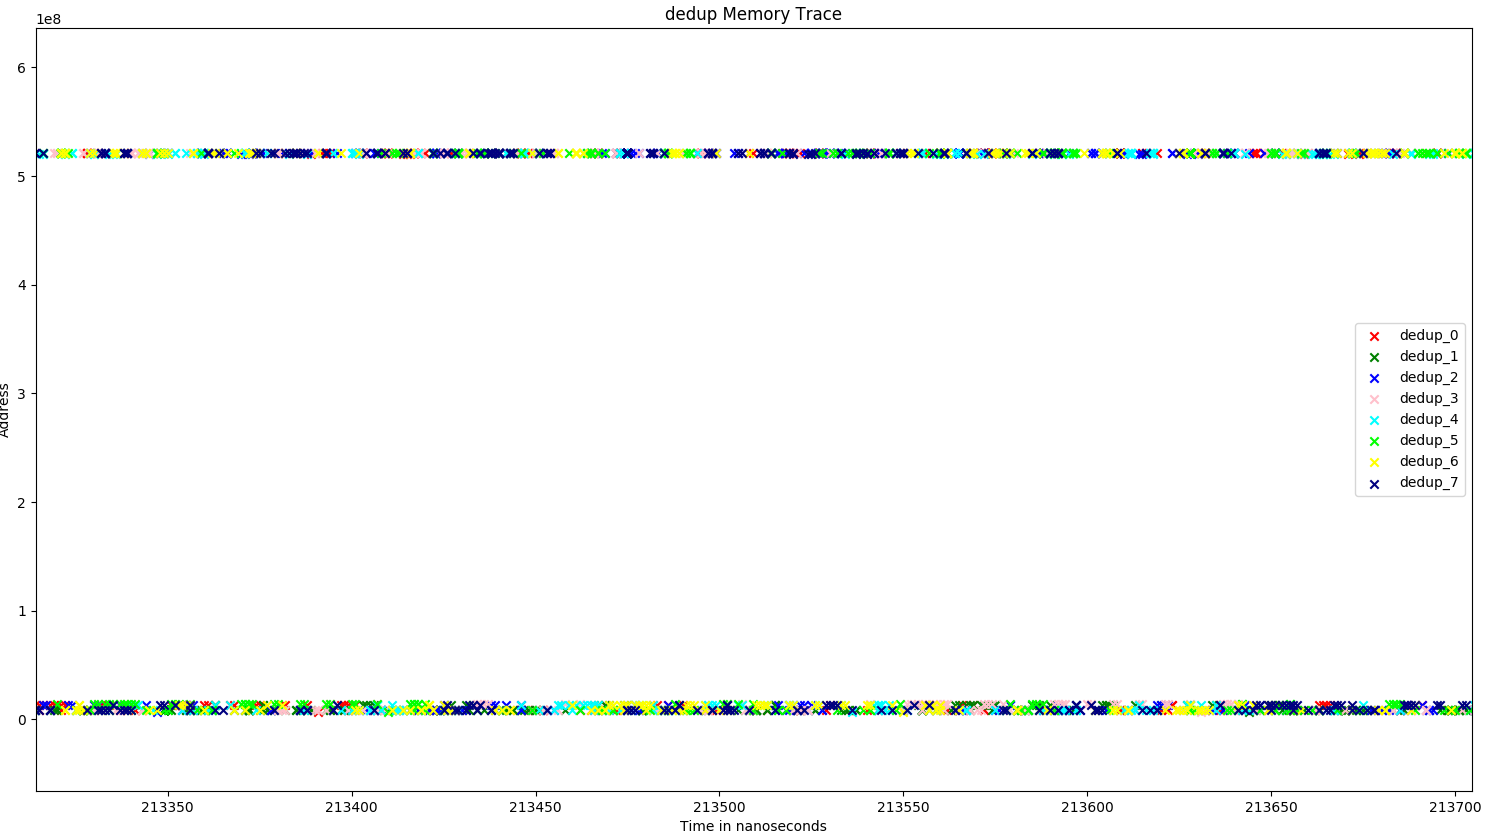
\includegraphics[width=\linewidth]{fig/dedup_dense.png}
		\caption{Memory Access from the Dedup PARSEC benchmark demonstrating the density of memory accesses}
		\label{fig:dedup_dense}
\end{figure}

The most important attributes of the memory traces as it relates to the proposed memory systems is the density of the traces, the overlap of the memory accesses between the processors, and how stationary the heavily utilized regions of memory are. The PARSEC benchmarks are sufficiently dense as illustrated by Figure~\ref{fig:dedup_dense}. It is clear from this image that there is heavily memory utilization during this section of the Dedup benchmark. On average across all processors, there is an average of 1.11 nanoseconds between memory accesses per core. The equates to an average of 2.22 cycles between memory access requests per processor as the processors are running at 2 Ghz. 


The location of the most heavily used memory region is stationary with respect to time for all PARSEC benchmarks. Figure~\ref{fig:dedup_whole} shows the whole of a Dedup memory trace. There are two major bands clear from this image, and the bands remain horizontal for the entirety of the plot indicating that these bands remain heavily accesses for duration of the trace. Figure~\ref{fig:dedup_dense} is a magnified view of the bottom band. This figure reveals that the bottom band is composed of two subbands which are also stationary with respect to time. The structure of the Dedup the memory trace is representative for all the PARSEC benchmarks. It is also clear from this image that the memory regions utilized by all of the processors overlap sufficiently to create bank conflicts.

\subsection{Ramulator}

We use the Ramulator DRAM simulator to compare the number of cpu cycles required to execute the PARSEC memory traces. We use the vanilla Ramulator simulator to acquire the baseline number of cpu cycles. We extended the memory controller in Ramulator in order to simulate the proposed memory system, and we use the modified Ramulator to examine the improvements the memory system has over the baseline. We use a consistant Ramulator configuration file so that the improvements we observe over baseline are purely a result of the memory system resolving bank conflicts. We test across two variables, the amount of memory overhead allowed by the memory system and the coded memory regions in the banks. 
The following are the specifics of the Ramulator configuration file used to acquire the simulation results:
\begin{itemize}
\item Standard : HBM
\item channels: 8
\item Ranks: 1
\item Speed: 1 Gigabits per second
\item Organization: 4 Gigabits
\item CPU ticks: 32
\item Memory ticks: 5
\end{itemize}
No caching was simulated.